% !TEX root = ../main.tex

\chapter{架构与模块设计}

\section{需求分析}
在进行架构设计和具体的模块设计之前,先对需求进行分析和总结。
这一小节将分析需要完成哪些设计和模型,来实现和验证在CIS芯片上的基于脉动阵列的ResNet18硬件加速运算。


\subsection{基础设定}
%由于整个芯片的顶层架构设计非常复杂,工作量也十分庞大。
%而本文的研究课题是一种CIS片上的深度学习神经网络运算的设计和建模。
%因此,这里可以做一些假设来代替非核心内容的设计工作。  

%首先,我们先假设使用的CPU、总线、DRAM、SRAM都是理想状态。
在本课题中,首先需要设计CIS芯片的基础架构。
CIS芯片的基础架构包括了CPU、总线、ROM、SRAM、DRAM以及图像数据信号通路上的各个模块。
CPU和总线是芯片上必不可少的设备。
但本课题中的深度学习算法的运算将全部由专门的硬件加速部件来完成运算,
因此下文将不再讨论CPU和总线的类型和设计。
关于存储设备,本课题将讨论选用存储器的种类和不同种类存储器所需要的存储大小。
因为通常在一些小型的CIS中,芯片所需的内存很少,所以只需要选用SRAM就可以满足系统的需要。
在考虑到深度学习神经网络的模型的大小,同时也参考了一些业内的深度学习神经网络运算专用芯片,本课题中的设计将同时使用SRAM和DRAM。

% 内存大小的设计

\subsection{详细需求}
%讨论详细需求。
% 用例


% 需求分析
因此,我们可以分解需求,并得到以下列出的需求点:
\begin{enumerate}
    \item CIS的基础模块
    \item 图像处理模块
    \item 脉动阵列的设计
    \item ResNet18在脉动阵列上的实现
\end{enumerate}

\section{总体架构设计}
CIS的顶层架构设计一般是由CPU、高速总线、存储以及数据通路上的各个外设组成。
这里只会在顶层架构设计中,描述上述部件的作用。
在后续的讨论中,将会把CPU、高速总线、存储器及数据通路上与深度学习计算无关的模块视作一些理想的设备,并做出一些假设。
本文将假设输入到深度学习运算模块的数据流,是一种理想的图像数据。
对于CIS上深度学习运算模块的设计,我们首先可以参考ISP芯片的设计逻辑。
因为我们可以将深度学习运算模块也视作一种图像处理的模块。



从图\ref{fig:top_arch}中可以看到这是经典的图像传感器与ISP以及其他功能部件连接在一条高速数据总线的结构。
总体架构可以分为几个部分:数据通路部分、系统控制部分和高速数据总线。
数据通路部分包含了IDA(Input Data Adapter)、深度学习神经网络加速模块、TX输出模块。
系统控制部分包含了CPU、DMA、Memory、SPI Flash以及其他外设模块(比如I2C和UART等接口模块)。
%TODO 架构图展示
\begin{figure}[htbp]
    \centering
    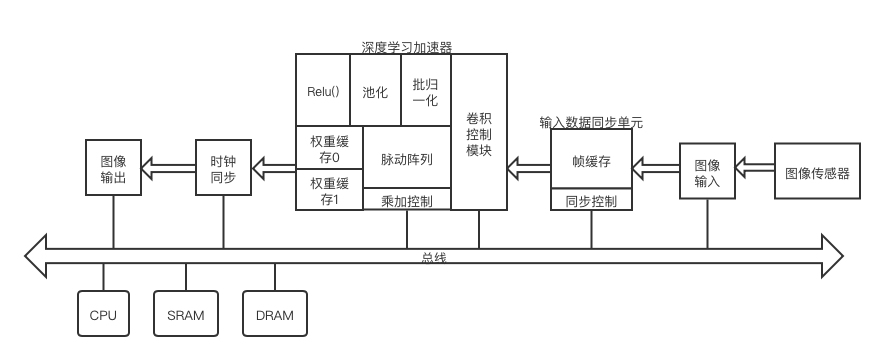
\includegraphics[width=15cm,height=6cm]{figures/top_arch.png}
    \caption{总体架构图}
    \label{fig:top_arch}
\end{figure}
%TODO 各个模块的简述
这里的视频数据格式设定为RGB888。

\section{CIS数据通路}
%TODO 展示Stream datapath的传输方式 sof eof href
%TODO DL accelerator在数据通路中的作用
%TODO Fix Timing模块做数据同步,最后输出结果
CIS芯片的作用,就是将图像传感器接收到的信号,转为数字信号后传输给后端。
CIS芯片上图像数字信号所经过的所有模块连接起来就像是一条单向的通道。
一般的,我们称这些模块所组成的通道为数据通路。
图像数据通路一般由输入、数据处理和输出三个部分组成。
通常地,这三个部分也具有各自不同的时钟域。

%TODO 架构图展示
\begin{figure}[htbp]
    \centering
    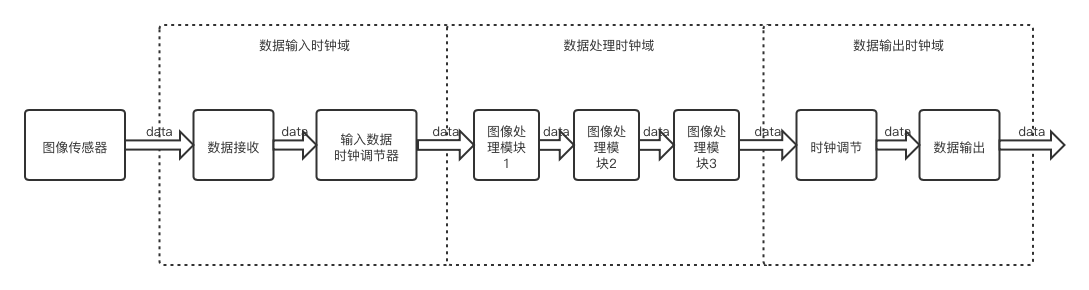
\includegraphics[width=15cm,height=5cm]{figures/datapath.png}
    \caption{图像信号处理的数据流图}
    \label{fig:datapath}
\end{figure}

%TODO 这里先描述以下datapath,包括DI、DP、DO三个时钟域。
如图\ref{fig:datapath}所示,图像处理部件的前后分别需要设置两个不同的时钟域用于输入和输出图像数据的信号。
因此,我们在设计CIS的数据通路中的深度学习运算模块时,也需要做相同的设计。
将输入模块的图像数据信号按一定的顺序排列好,按照脉动阵列的特性以一定的方式依次输入到阵列中。


在输入时钟域中,RX模块接收从CMOS传感器输出的数据。
由一个缓冲区暂存数据,经过时钟同步和一些预处理后向后面的数据处理时钟域输出数据。
在数据处理的时钟域中,深度学习运算模块将进行推理操作。
在输出时钟域中,FT(fix timing)模块将调整输出的时钟频率.TX模块负责以指定格式输出图像数据。  

\subsection{数据流的输入}
% TODO 
%   数据流的输入将由IDA(Input Data Adapter)模块处理。这个模块的主要作用是将Sensor输出的数据放到一个缓存区。
%   并将视频数据流的plck同步到数据流的时钟域。

这里假设从图像传感器输出的图像数据为224x224像素尺寸的图像。
视频数据流的输入需要参考流式设备的特性,合理的缓存大小和同步的时机是关键点。
对于卷积运算,缓存的行数大小应该大于等于卷积核的行数和列数之间的较大值。
例如,卷积核的尺寸为3x3时,缓存至少要保存3行数据。
如果,每帧图像的尺寸为224x224个像素点。
由RGB三个通道组成的每一帧都拆分成三个224x224x8比特。
那么需要给一个通道的一帧数据缓存的大小需要大于等于672个字节。

\begin{figure}[htbp]
    \centering
    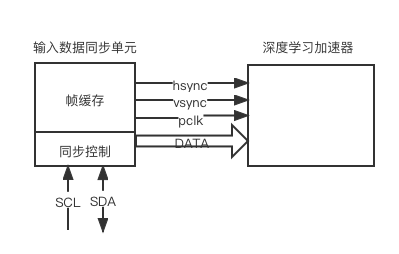
\includegraphics[width=12cm,height=8cm]{figures/input_data_adapter.png}
    \caption{输入数据同步单元架构图}
    \label{fig:input_data_adapter}
\end{figure}

上图\ref{fig:input_data_adapter}是数据输入同步单元与深度学习加速器之间的连线设计。
hsync用于行同步信号。
vsync用于帧同步信号。
pclk是像素时钟信号。
data是并行的图像数据,这里设定为8bit带宽。
SCL和SDA是用来读写模块寄存器的I2C接口的时钟信号和数据信号。




\subsection{数据流中的运算}
% TODO
% 在数据流中实时运算图像识别的算法

在数据通路中实时地进行图像识别的运算,是本设计的核心思想。
此设计选择了ResNet18作为实现的网络算法。
运算的模块将通过帧同步信号和行同步信号等机制来处理缓存的数据。
在实际应用时,将用于图像识别的人工智能处理器在物理位置上比较靠近图像来源(CMOS/CCD传感器),这样就避免了图像数据需要DRAM的存储。
另外,对于CNN算法,其中常用的一类CNN是共享权值的,这样权值的数量就不大,可以完整存放在片上SRAM中,从而使得权值也能避免存储在DRAM中。
这样处理后,整个系统就不需要DRAM做存储,从而大幅降低功耗。
设计3个缓存分别用于存储权值、输入数据、输出数据。
核心的运算模块是由最小运算单元组成的运算单元阵列。
普通的运算阵列受限于其规模。它的规模越大,需要的传输布线长度约长,传输时间越久,因此频率也无法做到很高。
这样的话,它的运算性能就会受到规模大小的限制。  


\subsubsection{ResNet18中的基本运算}
选择ResNet18在此设计中实现的主要原因是ResNet18结构简单且图像识别正确率出众。
除了一开始的7x7卷积核,在实现运算的BasicBlock中的卷积运算全部采用的3x3的卷积核。
这样既可以把如何进行卷积运算的设计表达清楚,也可以避免过多地描述卷积神经网络算法本身。

% TODO 简述ResNet18的网络结构
ResNet18由4个主要的残差层组成。
整个网络的开头,由7x7的卷积核做卷积运算和3x3的最大池化。
卷积运算有64个输出的通道。设定的步长是2,填充的边框是3。
最大值池化的步长是2,填充的边框是1。
最后输出的图像尺寸是112x112

之后是四个包含两个BasicBlock来做运算的残差层。
每个BasicBlock中都有两个3x3的卷积运算。
它们的深度不同,分别是64、128、256和512。
ResNet可能使用两种不同的残差单元。一种是BasicBlock,用于ResNet18和ResNet34这种浅层网络。
另一种是Bottleneck,用于50层及以上的ResNet。

\begin{codeblock}[language=python]
class BasicBlock(nn.Module):
    expansion: int = 1

    def __init__(
        self,
        inplanes: int,
        planes: int,
        stride: int = 1,
        downsample: Optional[nn.Module] = None,
        groups: int = 1,
        base_width: int = 64,
        dilation: int = 1,
        norm_layer: Optional[Callable[..., nn.Module]] = None,
    ):
        super().__init__()
        if norm_layer is None:
            norm_layer = nn.BatchNorm2d
        if groups != 1 or base_width != 64:
            raise ValueError("BasicBlock only supports groups=1 and base_width=64")
        if dilation > 1:
            raise NotImplementedError("Dilation > 1 not supported in BasicBlock")
        # Both self.conv1 and self.downsample layers downsample the input when stride != 1
        self.conv1 = conv3x3(inplanes, planes, stride)
        self.bn1 = norm_layer(planes)
        self.relu = nn.ReLU(inplace=True)
        self.conv2 = conv3x3(planes, planes)
        self.bn2 = norm_layer(planes)
        self.downsample = downsample
        self.stride = stride

    def forward(self, x: Tensor):
        identity = x

        out = self.conv1(x)
        out = self.bn1(out)
        out = self.relu(out)

        out = self.conv2(out)
        out = self.bn2(out)

        if self.downsample is not None:
            identity = self.downsample(x)

        out += identity
        out = self.relu(out)

        return out

\end{codeblock}

第一个残差层的卷积运算有64个输出通道。其输出的图像尺寸是56x56。
第二个残差层的卷积运算有128个输出通道。其中输出的图像尺寸是28x28。
第三个残差层的卷积运算有256个输出通道。其中输出的图像尺寸是14x14。
第四个残差层的卷积运算有512个输出通道。其中输出的图像尺寸是7x7。
最后,以平均池化、全连接和softmax结束整个resnet18网络。

下面使用pytorch来实现resnet18,以此来观察各个层之间的数据流。
\begin{codeblock}[language=python]
class ResNet18(nn.Module):
    def __init__(self, block, layers, num_classes=1000):
        self.inplanes = 64
        super(ResNet, self).__init__()
        self.conv1 = nn.Conv2d(3, 64, kernel_size=7, stride=2, padding=3,
                               bias=False)
        self.bn1 = nn.BatchNorm2d(64)
        self.relu = nn.ReLU(inplace=True)
        self.maxpool = nn.MaxPool2d(kernel_size=3, stride=2, padding=1)
        self.layer1 = self._make_layer(block, 64, layers[0])
        self.layer2 = self._make_layer(block, 128, layers[1], stride=2)
        self.layer3 = self._make_layer(block, 256, layers[2], stride=2)
        self.layer4 = self._make_layer(block, 512, layers[3], stride=2)
        self.avgpool = nn.AvgPool2d(7, stride=1)
        self.fc = nn.Linear(512 * block.expansion, num_classes)

        for m in self.modules():
            if isinstance(m, nn.Conv2d):
                n = m.kernel_size[0] * m.kernel_size[1] * m.out_channels
                m.weight.data.normal_(0, math.sqrt(2. / n))
            elif isinstance(m, nn.BatchNorm2d):
                m.weight.data.fill_(1)
                m.bias.data.zero_()

    def _make_layer(self, block, planes, blocks, stride=1):
        downsample = None
        if stride != 1 or self.inplanes != planes * block.expansion:
            downsample = nn.Sequential(
                nn.Conv2d(self.inplanes, planes * block.expansion,
                          kernel_size=1, stride=stride, bias=False),
                nn.BatchNorm2d(planes * block.expansion),
            )

        layers = []
        layers.append(block(self.inplanes, planes, stride, downsample))
        self.inplanes = planes * block.expansion
        for i in range(1, blocks):
            layers.append(block(self.inplanes, planes))

        return nn.Sequential(*layers)

    def forward(self, x):
        x = self.conv1(x)
        x = self.bn1(x)
        x = self.relu(x)
        x = self.maxpool(x)

        x = self.layer1(x)
        x = self.layer2(x)
        x = self.layer3(x)
        x = self.layer4(x)

        x = self.avgpool(x)
        x = x.view(x.size(0), -1)
        x = self.fc(x)

        return x

\end{codeblock}


% TODO 展开conv1~conv5的详细流程
根据上面的ResNet18的架构分析,我们可以将整个计算过程详细展开。
首先,输入的图像数据是224x224x3的尺寸。
数据经过了卷积核尺寸为7x7的卷积运算。其中,步长为2,边框的填充为3。
得到了尺寸为112x112x64的特征图。
% TODO 展开7x7卷积运算。
% TODO 



将特征图经过批归一化和Relu()激活函数。这两个运算不会改变特征图的维度。
% TODO 展开BN和Relu激活函数


之后用3x3的卷积核将特征图进行最大池化,步长为2,边框填充为3,得到56x56x64的特征图。
% TODO 展开3x3的maxpooling


后面就开始将数据依次输入4个残差层。
% TODO 展开残差层的计算
残差层包含了两个BasicBlock。因此它的运算可以参考上面的代码段中BasicBlock类的内容。
首先,输入从上一层得到的56x56x64的特征图。
将这个特征图用3x3x64的卷积核做卷积运算。使用的步长为1,填充的边框为1,得到56x56x64的特征图输出。
假设输入的特征图大小为m,卷积核大小为x,步长为s,边框填充层数为p,那么输出的特征图大小 $m^{'}$ 由公式(2-1)计算得到:
\begin{equation}
m^{'} = \frac{( m + 2 \times p - x )}{s} + 1 
\end{equation}



\subsection{运算模块}
前文讲到,普通的运算方法受限于深度学习神经网络结构的规模影响。
本设计中,将设计一种基于脉动阵列的卷积运算来改善这个问题。
%TODO ResNet18的Basic Block
%TODO x -> conv3x3 -> BN -> Relu -> conv3x3 -> BN ( + 入口的x)-> out -> Relu -> out
%TODO x -> conv7x7,stride=3,padding=3 -> BN -> 



%TODO 脉动阵列实现矩阵乘法的CMODEL
脉动阵列是1978年KUNG H T提出的一种应用在片上多处理器的体系结构。它是由多个相同的、结构简单的计算单元
以网状形式连接而成的,具有并行性、规律性和局部通信的特征。在深度残差网络ResNet18中,由5个卷积层组成,
除了第一个卷积层外,后4个卷积层都是由2个基础块组成。基础块的结构如下图x所示。其中的批量标准化和Relu函
数都可以设计专用的运算模块,而3x3的卷积运算可以通过脉动阵列来运算。 
%REF KUNG H T, Leiserson C E. Systolic arrays(for VLSI)[C]. Sparse Matrix Proceedings 1978, Society for Industrial and Applied Mathematics, 1979.

\begin{table}[!hpt]
    \bicaption[PE的寄存器表]{PE的寄存器表}{Register Table Of PE}
    \label{tab:firstone}
    \centering
    \begin{tabular}{@{}lllr@{}} \toprule
        Type & Name & Description & Size \\ \midrule
        input  & CLK  & 输入PE模块的时钟信号 & 32b \\
        input  & RST  & 模块重置寄存器 & 16b \\
        input   & SCLR   & 同步清零寄存器 & 16b \\
        input   & A   & 输入参数A & 8b \\
        input   & B   & 输入参数B & 8b \\
        output   & Next\_A   & 输出到下一个PE的A & 8b \\
        output   & Next\_B   & 输出到下一个PE的B & 8b \\
        output & P & PE的运算结果P & 16b \\ \bottomrule
    \end{tabular}
  \end{table}

  
脉动阵列的设计和C模型实现,可以分为两个部分:脉动阵列模块的顶层设计和处理单元的设计。
处理单元(PE)的寄存器:时钟、重置、同步清零、输入参数A、输入参数B、输出给下一级的A、输出给下一级的
B、输出P值。


脉动一词来源于心血管。
在冯诺依曼的计算机体系中,指令和数据是一起存储在存储器中。
在运算的过程中,数据从存储器中被取出,经过处理器的处理后再写回到存储器中。
这个过程就像是人体的血液循环一样,因此得名脉动。  
\begin{figure}[htbp]
    \centering
    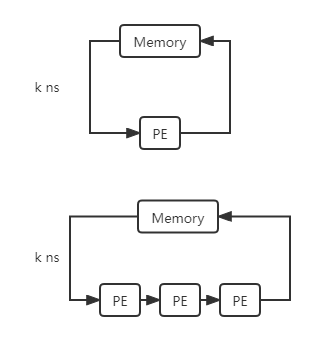
\includegraphics[]{figures/systolic_array.png}
    \caption{脉动阵列原理图}
    \label{systolic}
\end{figure}  
当运算的过程是由多个可重复的运算单元组成时,每一个运算单元都会与一个或者多个周围的单元发生数据交互,结果或将存储在运算单元内部,或将传递给下一个单元。
在脉动阵列中,最重要的是设计一种在运算单元之间联系的规则,并且把高层次的算法映射到每一个单元上。
脉动阵列的优势如图2-2所示,在某种计算需要计算单元迭代执行3次时,可以减少(3-1)次的存储器读写时间。
这里的脉动阵列是使用乘累加器作为其处理单元的。
它非常适合如矩阵运算,卷积等等数据流具有一定规律的算法。  

在分析了ResNet18的网络结构以后,下面将会把所有网络中涉及到的运算分别列出并展开分析。
通过这样的分析,可以得到所有的运算模块需求。
具体的运算模块需求如下:
\begin{enumerate}
    \item 边框填充(padding);
    \item 基于脉动阵列的2维卷积运算;
    \item 最大池化;
    \item Relu函数;
    \item 批归一化;
\end{enumerate}

\subsubsection{边框填充(padding)和数据输入}
对于边框填充,如果直接对输入数据进行修改,将会需要很大的存储来缓存数据,并且不排除会有很多读写的操作影响整个运算的效率。
因此,我们需要设计一个专门用于填充边框的模块。
让它在把数据送入脉动阵列的通道以前,加入对应的填充值。
在把数据送入脉动阵列时,需要将数据按照执行卷积运算时的顺序依次送入脉动阵列。
下图是一个对一个5x5的输入用2个3x3的卷积核做卷积运算的示意图,用来说明怎样对输入脉动阵列的数据进行排序和分组的。
图中,左侧的由两位数字组成的标号表示了它在5x5的矩阵中的位置。
右侧的两列分别是W0和W1的两个卷积核的数据平铺展开得到的。
0到8的编号表示了它们在两个卷积核中的位置。
%这里插入一个对一个5x5的输入用3x3的卷积核做卷积运算的示意图

\begin{figure}[htbp]
    \centering
    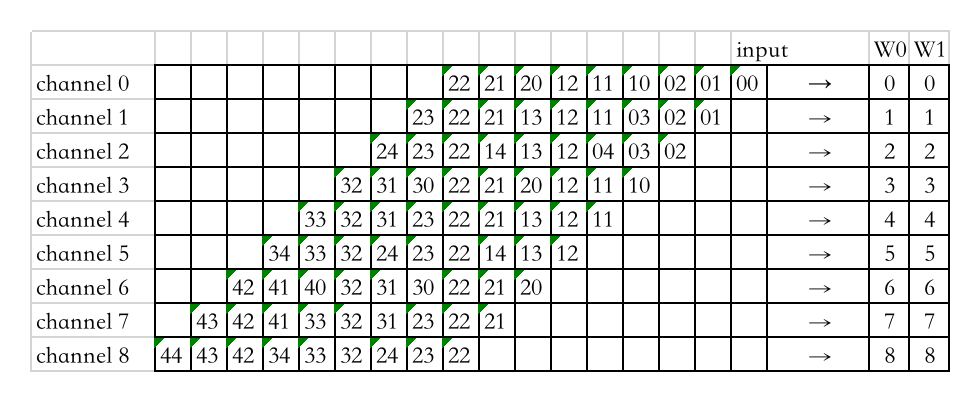
\includegraphics[width=15cm,height=7cm]{figures/input_systolic_array.png}
    \caption{数据输入脉动阵列示意图}
    \label{systolic}
\end{figure}





\section{已知的深度学习神经网络运算单元}

% TODO CPU和GPU平台上的加速运算
在常见的CPU和GPU平台上,SIMT和SIMD等技术被广泛地应用。
从字面上解释,SIMT是单指令多线程,而SIMD为单指令多数据流。
在SIMD中,向量中的元素处在相同的地址空间。
而SIMT中的每一个线程的寄存器都是私有的。可以通过共享内存或是其他的线程内同步机制来进行通信。

\subsection{影响因子和依据}
在开始设计深度学习神经网络的运算模块之前,本章节将提出一些影响设计的因素,并描述如何将这些因素考虑在内来帮助我们完成设计。
其中精准度、吞吐量、延迟、能效比和功耗,都是衡量深度学习神经网络运算的硬件单元的最重要因素。


% TODO 精确度 吞吐量和延迟 能效比和功耗
准确度是这类问题中最常见的一个指标。对于图像分类问题,准确度报告为正确分类图像的百分比,而对于目标检测问题,精度报告为平均准确度。
影响准确性的因素包括任务的难度和数据集。因此,准确度在建模的过程中将被用来验证设计的正确性。
吞吐量用于指示在给定时间段内可以处理的数据量或可以完成的任务的执行次数。高吞吐量通常是应用程序的关键。
延迟度量输入数据到达系统和生成结果之间的时间。低延迟对于实时交互应用程序(如虚拟现实、自主导航和机器人技术)是必要的。
吞吐量和延迟通常被认为是可以直接相互派生的。
一般的,在给定能量单位下可处理的数据量或完成任务的执行次数被称为能效比。


\subsection{基于脉动阵列的深度残差网络}
本文中将基于脉动阵列来实现深度残差网络。







% \begin{table}[!hpt]
%     \caption[PE的寄存器表]{PE的寄存器表}{Register Table Of PE}
%     \label{tab:firstone}
%     \centering
%     \begin{tabular}Type & Name & Description & Size \\  \toprule
%       input & CLK  & 输入PE模块的时钟信号 & 32b \\ \midrule
%       input & RST  & 模块重置寄存器 & 16b \\
%       input & SCLR & 同步清零寄存器 & 16b \\
%       input & A & 输入参数A & 8b \\
%       input & B & 输入参数B & 8b \\
%       output & Next_A & 输出到下一个PE的A & 8b \\
%       output & Next_B & 输出到下一个PE的B & 8b \\
%       output & P & PE的运算结果P & 16b \\ \bottomrule
%     \end{tabular}
% \end{table}  



\section{存储}
%TODO 关于存储Multiple Bank的设计(状态机)
本设计中,专门对存储进行了优化,区分开了不同的RAM区域来存储不用的数据,主要由以下几个区域:存储输入和输出数据的
INRAM和OUTRAM、存储网络数据的NRAM、存储权重的WRAM、存储系统数据的SRAM以及存储临时数据的TRAM。拆分存储的设计
主要有以下两大好处:读写的带宽和避免冲突。
拆分存储之后,SRAM可以被调整为适当的读写宽度。假设输入和输出的宽度是$X_a \times K$字节,存储网络和权重数据的
NRAM和WRAM为$X_a \times X_a \times K$字节。如果是用CPU或GPU,且未做优化的情况下,处理器只能按照固定宽度读取
数据。

DRAM和SRAM
先进的存储技术可以降低高密度存储器(如DRAM)的访问能量。
例如,嵌入式DRAM(eDRAM)在芯片上提供高密度存储器,以避免关闭芯片电容的高能耗成本[97];eDRAM的密度比SRAM高2.85倍,能效比DRAM高321倍(DDR3)[93]。
与DRAM相比,eDRAM还提供了更高的带宽和更低的延迟。在DNN处理中,eDRAM可用于在芯片上存储数十兆字节的权重和激活,以避免芯片外访问,如DaDianNao[93]所示。
eDRAM的缺点是其密度低于片外DRAM,并且会增加芯片成本。
DRAM也可以使用硅通孔(TSV)堆叠在芯片顶部,而不是将DRAM集成到芯片本身。
这项技术通常被称为三维存储器,并已以混合存储立方体(HMC)[98]和高带宽存储器(HBM)[99]的形式商业化。
3-D内存提供了一个数量级的更高带宽,并且相对于现有的2-D DRAM,访问能量减少了5倍,因为TSV的电容低于典型的片外互连。
最近的工作探索了使用HMC以多种方式高效处理DNN。例如,Neurocube[100]将SIMD处理器集成到HMC的逻辑芯片中,使内存和计算更紧密地结合在一起。
Tetris[101]探讨了HMC与Eyeris空间架构和行固定数据流的结合使用。
它建议分配比片上存储器更多的计算区域(即更大的PE阵列和更小的全局缓冲区),以利用HMC的低能量和高吞吐量特性。它还调整数据流,以考虑HMC内存和更小的片上内存。
Tetris在使用传统2-D DRAM的基线系统上实现了1.5倍的能耗降低和4.1倍的吞吐量增加。

SRAM不是将内存放在计算附近,而是将计算放在内存中。
例如,乘法和累积操作可以直接集成到SRAM阵列的位单元中[102],如图36(a)所示。
在这项工作中,使用5位DAC将字线(WL)驱动到表示特征向量的模拟电压,而位单元存储二进制权重±1。
比特单元电流(IBC)实际上是特征向量的值和存储在比特单元中的权重的值的乘积;来自列中位单元的电流加在一起对位线(VBL)放电。
与从SRAM读取1位权重并单独执行计算相比,该方法可节省12倍的能量。
为了对抗电路的非理想性,DAC考虑了关于WL电压的非线性位线放电,并使用升压来组合易受设备变化影响的弱分类器,以形成强分类器[103]。

非易失性电阻存储器
乘法和累积操作也可以直接集成到高级非易失性高密度存储器中,方法是将其用作可编程电阻元件,通常称为忆阻器[105]。
具体地,如图36(b)所示,以电阻器的电导作为权重,以电压作为输入,以电流作为输出,执行乘法。
加法是通过将不同忆阻器的电流与基尔霍夫电流定律相加来完成的。这是权重固定数据流的最终形式,因为权重始终保持在适当的位置。
这种方法的优点包括:由于计算被嵌入内存中,从而减少了数据移动,因此降低了能耗;由于内存和计算可以以与DRAM类似的密度进行密集封装,因此增加了密度[106]。
非易失性电阻存储器器件有几种常见的候选器件,包括相变存储器(PCM)、电阻RAM(RRAM或ReRAM)、导电桥RAM(CBRAM)和自旋转移转矩磁RAM(STT-MRAM)[107]。
这些设备在耐久性(即可以写入多少次)、保留时间、写入电流、密度(即单元大小)、变化和速度方面有不同的权衡。
如[108]所述,使用非易失性电阻存储器进行处理有几个缺点。
首先,它受到前面描述的模拟处理的精度降低和ADC/DAC开销的影响。
第二,阵列尺寸受到连接电阻器件的导线的限制;具体而言,对于大型阵列(例如1k×1k),导线能量占主导地位,并且沿导线的红外压降会降低读取精度。
第三,对电阻器件进行编程的写入能量可能非常昂贵,在某些情况下需要多个脉冲。
最后,电阻器件还可能受到器件间和周期间变化的影响,在整个电导范围内具有非线性电导。


